\chapter{A New Theoretical Formalism}

In this chapter, a formalism that describes the wobbling properties in odd-$A$ nuclei will be presented. The model was developed recently by the current team (i.e., Raduta and Poenaru) and applied to $^{135}$Pr \cite{raduta2020new}, and the `Lu family' with $^{161,165,167}$Lu \cite{raduta2020approach} and $^{163}$Lu \cite{raduta2020approach,raduta2020towards,poenaru2021parity,poenaru2021extensive1,poenaru2021extensive2}. This framework is an original contribution to the field of nuclear structure, with focus on the theoretical aspects of collective phenomena in nuclei.

\section{Previous Work - Foundation}

From a development standpoint, it is instructive to review the previous `stages' that lead to the current work, since the description of odd-$A$ nuclei achieved in here is strongly connected with former calculations done by the team. Consequently, in this section a brief overview of the wobbling motion in $^{163}$Lu done by Raduta et al. in 2017 \cite{raduta2017semiclassical} will be given. Indeed, by using a \emph{semi-classical} approach, the wobbling properties of this odd-mass isotope were accurately described. 

The semi-classical approaches tend to be very useful when applied to problems having a \emph{quantal} Hamiltonian that contains quantities which behave as in the \emph{classical limit} when certain constraints or approximations are made. Moreover, these methods always keep the dynamics of the system in close contact with the classical features, which in principle are easier to interpret (i.e., a clear physical meaning). For this reason, the collective properties of $^{163}$Lu were characterized by such a method. Dealing with an odd nucleus it makes sense to adopt a Particle + Rotor Model in which the odd quasi-particle couples to an even-even core. From the total Hamiltonian $H=H_\text{rot}+H_\text{sp}$ (recall discussion on the PRM model \ref{triaxial-prm-general-hamiltonian} and also QTR Hamiltonian \ref{oddA-QTR-general-hamiltonian}), one obtained the energy spectrum for the four wobbling bands in this nucleus. Remarking the fact that there is another debate regarding the `true' nature of the fourth triaxial strongly-deformed band. For example, Jensen et al. \cite{jensen2004coexisting} suspect that this band is built from single-particle excitations, meaning that the states to not show wobbling mechanism. However, Tanabe et al. \cite{tanabe2008selection} is in favor of attributing $n_w=3$ for TSD4. More details on the interpretation of TSD4 will be discussed in the following sections.

After the initial Hamiltonian problem was established, classical equations of motions which fully describe the motion of $\mathcal{Q}$ and $\mathscr{C}$ (recall notations from Table \ref{notation-table-wobbling} that will still be used throughout the remaining chapters) are obtained through the Variational Principle (VP) by following a textbook procedure. The procedure of applying VP translates to the \emph{dequantization} procedure of an initial quantal Hamiltonian, thus making the change from a quantum space $S_\text{qt}$ to a classical space $S_\text{cls}$. This kind of transition $S_\text{qt}\to S_\text{cls}$ was also used previously for describing collective phenomena \cite{raduta2007semiclassical,chen2016two,budaca2018tilted}. For keeping a short overview of the foundational stage, the VP method applied to $H$ is skipped for now, but it will be detailed in a subsequent section. Furthermore, the classical equations of motions were solved with several restrictions, and the energy spectrum was analytically obtained (see Eq. 3.23 from the same reference). The excited bands TSD2, TSD3, and TSD4 were constructed via a phonon operator (denoted by $\Gamma_1^\dagger$ in Eq. 3.43 from \cite{raduta2017semiclassical}, which acts every state $I$). This approach makes it possible to have $n_w=3$ phonon excitations that are obtained by applying the phonon operator three times on the spin states belonging to the yrast band TSD1. In fact, since the states from TSD4 have negative parity, they are obtained by applying twice $\Gamma_1^\dagger(\pi=+1)$ and once $\Gamma_1^\dagger(\pi=-1)$, where the former phonon has positive parity and the latter has a negative parity. A schematic representation with the mechanism of action for the phonon operator from this formalism is shown in Fig. \ref{phonon-operator-schematic}.
\begin{figure}
    \centering
    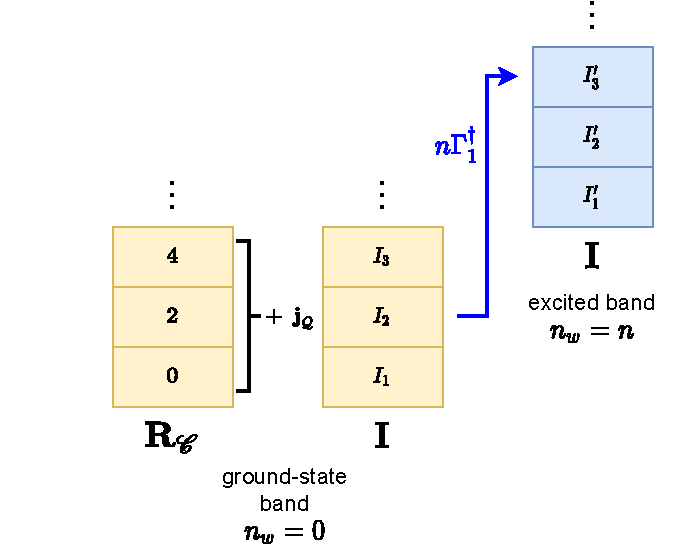
\includegraphics[width=0.75\textwidth]{Chapters/Figures/w0_phonon_operator.pdf}
    \caption{The mechanism of action for the phonon operator introduced in Ref. \cite{raduta2017semiclassical} for creating excited states of a given angular momentum, from the ground state bands. The core's angular momentum is defined as $\mathbf{R}_\mathscr{C}$, while the quasi-particle a.m. is denoted by $\mathbf{j}_\mathcal{Q}$. The ground-state band (yrast) emerges from the coupling of the quasi-particle with the triaxial core, giving rise to a series of spins $I_i=R_i+j$. By acting with $\Gamma_1^\dagger$ $n$-times on any of these states, then an excited level is obtained in a $n_w=n$ wobbling band. Keep in mind that one phonon operator increases the spin of a state by one unit.}
    \label{phonon-operator-schematic}
\end{figure}


From the seminal work from 2017 of the team, several features are emphasized:
\begin{itemize}
    \item The four TSD bands are considered as zero-, one-, two-, and three-wobbling phonon bands for TSD1, TSD2, TSD3, and TSD4, respectively
    \item Each excited band is obtained by acting on the yrast (TSD1) band with one-, two-, and three-phonons, respectively (e.g., a state $I$ from TSD2 is obtained by acting with the wobbling-phonon operator on a state $I-1$ from TSD1 and so on), according to Fig. \ref{phonon-operator-schematic}
    \item Wobbling structure for the group TSD1-2-3 emerged from a proton $i_{13/2}$ ($\mathcal{Q}_p$) where all spin states have positive parity
    \item The band TSD4 has spin states with negative parity, and it is built on a proton from the $h_{9/2}$ orbital (also a $\mathcal{Q}_p$)
    \item In the expression of the rotor Hamiltonian, the rigid-like MOI were adopted (see Eq. \ref{eq-irrotational-rigid-mois}) which depend on $\gamma$ and $\mathcal{I}_0$
    \item Analytical expressions for the energies were expressed in terms of total spin and wobbling phonon numbers
    \item Experimental data was reproduced through a fitting procedure, with the free parameters $\mathcal{I}_0^{-1}$ (rotor part) and a \emph{scaling factor} $s=V\cdot \mathcal{I}_0$ (single-particle part)
    \item The model assumes similar MOI across all four bands
    \item Deformation parameters $\beta_2$ and $\gamma$ were a priori fixed (taken from literature)
\end{itemize}

A year later, the team also extended this method into analyzing the wobbling properties of two more isotopes: $^{165,167}$Lu \cite{raduta2018wobbling}, and the model showed again that it was an useful tool in providing a realistic description of the wobbling motion in odd-mass nuclei. Hereafter, when referring to the procedure realized by Raduta and Poenaru in \cite{raduta2017semiclassical} and \cite{raduta2018wobbling}, the term $\mathbf{W_0}$ will be used. Throughout the following chapters, comparisons between the newly developed and improved theory and $\mathbf{W_0}$ will be made when necessary, in order to understand several key differences.

\section{Re-interpretation of The Wobbling Motion}

The $\mathbf{W_0}$ formalism can be regarded as a cornerstone in the description of an odd-$A$ particle-triaxial-rotor system done by the team. In a more recent follow-up work (2020) done by Raduta and Poenaru \cite{raduta2020approach,raduta2020towards}, a new interpretation of the wobbling bands was made, relative not only to the odd-$A$ $^{163}$Lu, but to an entire set of wobblers. The way of obtaining yrast and excited states within the collective spectrum turned out to be a first within literature, especially for $^{163}$Lu and $^{135}$Pr, since these nuclei have been drawing a lot of attention lately. The model starts with the typical QTR Hamiltonian:
\begin{align}
    \hat{H}=\hat{H}_\text{rot}+\hat{H}_\text{sp}\ ,
    \label{total-ham-approach-w1}
\end{align}
where $\hat{H}_\text{sp}$ represents the quasi-particle that moves inside the quadrupole mean-field as described in Eqs. \ref{eq-nilsson-ham-spherical-harmonics} and \ref{single-particle-nilsson-defored-potential} (recall discussion on the $\gamma$-deformed Nilsson potential and also Sections \ref{trm-model} - \ref{tprm-model}):
\begin{align}
    \hat{H}_\text{sp}=\epsilon_j+\frac{V}{j(j+1)}\left[\cos\gamma\left(3j_3^3-\mathbf{j}_\mathcal{Q}^2\right)-\sqrt{3}\sin\gamma\left(j_1^2-j_2^2\right)\right]\ ,
    \label{single-particle-ham-approach-w1}
\end{align}
with $\epsilon_j$ is the intrinsic energy of the particle from the corresponding $j$-shell (as it was discussed in Section \ref{tprm-model}). The total angular momentum of the odd-particle + core system is $\mathbf{I}=\mathbf{R}_\mathscr{C}+\mathbf{j}_{\mathcal{Q}_p}$. The components of the total angular momentum are: $$\mathbf{I}=\{\hat{I}_1,\hat{I}_2,\hat{I}_3\}\ ,$$ while the a.m. components for the $\mathcal{Q}_p$ are given as $$\mathbf{j}_{\mathcal{Q}_p}=\{\hat{j}_1,\hat{j}_2,\hat{j}_3\}\ .$$ The axes labelling for the triaxial ellipsoid is $(1,2,3)$. Knowing this, one can express the rotor part as:
\begin{align}
    \hat{H}_\text{rot}=\sum_{k=1}^3A_k(\hat{I}_k-\hat{j}_k)^2\ ,
    \label{rotor-ham-approach-w1}
\end{align}
where the inertial factors $A_k$ are expressed in terms of the three MOI:$$A_k=\frac{1}{2\mathcal{I}_k}\ .$$
Note that the Hamiltonian from Eq. \ref{rotor-ham-approach-w1} is just as the one expressed in Eq. \ref{general-rotor-hamiltonian}, except that here, the components of $\mathbf{R}_\mathscr{C}$ are given in terms of $\mathbf{I}$ and $\mathbf{j}_{\mathcal{Q}_p}$.

Obviously, the next task would be to obtained the eigenvalues of the Hamiltonian, which would comprise the energies of the system. One can proceed with the diagonalization procedure of $\hat{H}$ using a set of states that manifest the invariance to rotation by $\pi$ around a particular axis (the $D_2$ symmetry), since the Hamiltonian exhibits such a property. However, it is more practical to describe the system only though a few variables that have a classical counterpart. By doing this, the system dynamics will be close to the classical analogy of a rotating body lacking axial symmetry. The semi-classical approach that best fits this need os the Time-Dependent Variational Principle (TDVP), to which one associates the Time-Dependent Variational Equation (TDVE). When applying this Variational Principle on an initial problem, the requirement is to have a variational state which is constructed carefully, such that it embeds the necessary degrees of freedom of the underlying physics. Furthermore, VP will provide the time dependence of the variables that comprise the variational state itself \cite{budaca2018tilted}. Additionally, for each variable that parametrizes the state (usually the variables are complex), the TDVE will provide its equation of motion, thus finding the `connection' between the initial quantal variable (belonging to $S_\text{qt})$ and the classical variable (belonging to $S_\text{cls}$).

The discussion regarding the TDVP and TDVE from above can therefore be summarized in the following equation, which must be associated to the quantum Hamiltonian ($\hat{H}\in S_\text{qt}$) defined in Eq. \ref{total-ham-approach-w1}:
\begin{align}
    \delta\int_0^t\bra{\Psi_{IjM}}\hat{H}-i\frac{\partial}{\partial t'}\ket{\Psi_{IjM}}dt'=0\ .
    \label{tdve-approach-w1}
\end{align}
Obviously, the variational state $\ket{\Psi_{IjM}}\equiv\Psi_\text{trial}$ (also known as the \emph{trial function}) must be chosen in such a way that it comprises the entire space $S_\text{qt}$ of the original quantal Hamiltonian. This can be achieved if $\Psi_\text{trial}$ is a \emph{coherent state} \cite{glauber1963coherent}, which due to its \emph{completeness} property, will span all the basis vector states from $S_\text{qt}$. Keep in mind that for $S_\text{qt}$ the states belong to the Hilbert space of $\hat{H}$. For the present case, the trial function is defined as:
\begin{align}
    \Psi_\text{trial}\equiv\Psi_{IjM}=\mathcal{N}e^{z\hat{I}_-}e^{s\hat{j}_-}\ket{IMI}\ket{jj}\ ,
    \label{trial-function-appeoach-w1}
\end{align}
where the ladder operators for the total and single-particle a.m. are represented by $\hat{I}_-$ and $\hat{j}_-$, respectively. The factor $\mathcal{N}$ is the normalization constant, which keeps the trial function normalized to unity. Its value is given by \cite{raduta2007semiclassical,raduta2020new}:
\begin{align}
    \mathcal{N}=\left(1+|z|^2\right)^{-2I}\left(1+|s|^2\right)^{-2j}\ .
\end{align}
The states that are involved in $\Psi_\text{trial}$ are as follow: $\ket{IMK}$ represent the Wigner-D functions (i.e., eigenstates of $\hat{I}^2$ and $\hat{I}_3$), while $\ket{j\Omega}$ are the wave-functions of the odd quasi-particle $\mathcal{Q}$ (the eigenstates of $\hat{j}^2$ and $\hat{j}_-$). Notice that for both cases, the trial function contains their extremal form, namely the states of maximum projections $(K=I,\Omega=j)$. For $\ket{IMK}$, one has:
\begin{align}
    \ket{IMK}&=\sqrt{\frac{2I+1}{8\pi^2}}\mathcal{D}_{MK}^I \nonumber\\
    \ket{IM-K}&=\sqrt{\frac{2I+1}{8\pi^2}}\mathcal{D}_{M-K}^I\ .
    \label{IMK-wigner-functions}
\end{align}
The second equation denotes the \emph{time-reversed} states, which are obtained by changing the projection $K$ to $-K$. The single-particle states can be defined more generally as:
\begin{align}
    \ket{\chi_\mathcal{Q}}&=\sum_{j\Omega}c_{j\Omega}\ket{j\Omega}\nonumber\\
    \ket{\bar{\chi}_\mathcal{Q}}&=\sum_{j\Omega}c_{j-\Omega}\ket{j-\Omega}\ ,
    \label{j-Omega-single-particle-states}
\end{align}
where the wave-function is expressed in terms of the projections $\Omega=-j,\dots,j$. Obviously the single-particle also has time-reversed states and moreover, $\ket{\bar{\chi}_\mathcal{Q}}$ is degenerate with $\ket{\chi_\mathcal{Q}}$. Because of the $D_2$ symmetry for $\hat{H}$, the total wave-function can be formulated as the a sum over the components $K, \Omega$ and over $j$. Denoting the total wave-function of the odd-mass nucleus as $\ket{\Psi}_\text{odd}$ (not to be confused with the trial function $\Psi_\text{trial}$), it must comprise both the intrinsic and the single-particle degrees of freedom, namely:
\begin{align}
    \ket{\Psi_\text{odd}}=\ket{\Psi_\text{intr.}}\otimes\ket{\Psi_\mathcal{Q}}\ .
    \label{total-wavefunction-oddA-general}
\end{align}